\chapter{Interaktiv planlægning}
\label{chap:is}
\fxwarning{Mangler Evaluering}
\fxwarning{Mangler Opsummering}
Interaktiv planlægning (\is) er det sidste anvendelsesområde vi vil belyse med henblik på at indføre tid i \pycsp. Det har dog vist sig at emnet kun er sparsomt berørt i litteraturen, og der er ikke en klar definition på hvad det er og hvor det anvendes. 
%og at de få definitioner af \is vi har fundet, ikke er et selvstændigt anvendelsområde, men en definition af RTP med en hard deadline uden at være et kritisk system. \cite{?}. 
Vi forventede at dette anvendelsesområde var brugt i forbindelse med computerspil, men efter at have studeret litteraturen, og have rådført os med Lektor Kenny Erleben, der underviser på Det Danske Akademi for Digital Interaktiv Underholdning (DADIU), er vi kommet frem til der ikke findes en udbredt definition af \is. Han fortæller desuden at en af begrundelserne for at computerspilfirmaerne ikke er interesseret i at oplyse om deres metoder til at planlægge begivenheder i spil, er at det  betragtes som en  virksomhedshemmelighed. 

Vi vil derfor i stedet på baggrund af en række praktiske eksempler indkredse hvad vi forventer \is skal kunne bruges til, og på baggrund af eksemplerne se på muligheden for at implementere en model, så eksemplerne kan implementeres i \pycsp. Dette kapitel adskiller sig dermed væsentligt fra de foregående to kapitler, i og med tidsmodellen ikke baserer sig på en fast definition givet af litteraturen og vi ikke bygger på kendt viden.

\section{Eksempler}
Vi har valgt to scenarier som vi forventer med fordel kan benytte \is. Det første er en repræsentation af et ur, hvilket vi mener er det simpleste eksempel der kan gøre brug af \is. Det andet eksempel er en del af et computerspil, som er vores forventede primære anvendelsesområde for \is. 

\subsection{Et ur}
Det første eksempel på \is er en repræsentation af et digitalur. Uret består af seks cifre, og en gang i sekundet skal sekunderne tælles op. Det er et  krav at en opdatering af uret skal sætte uret til at vise det korrekte tidspunkt. Vi forestiller os at uret er en del af et større system hvor der er andre ressourcekrævende begivenheder der er vigtigere at få udført end opdateringen af uret. Opdatering af uret foregår ved at planlægge en begivenhed til hvert sekund, der specificerer hvad uret skal vise. Da det har en lav prioritet, er der ikke er nogen garanti for at denne begivenhed indtræffer i det sekund den er planlagt til. Derfor skal begivenheden  bortkastes såfremt den overskrider sin deadline. Deadlinen vil være det når et nyt sekund begynder, for at sikre den krævede korrekthed. 

Uret er repræsentativt for \is da der planlægges en række begivenheder der skal foregå i fremtiden, og hvor hver begivenhed også har tilknyttet en deadline.

\subsection{Computerspil}
Et andet eksempel vi mener repræsenterer  \is, er mere realistisk og bunder i vores oprindelige forventning om at \is  var defineret af computerspilindustrien, som en metode til at planlægge hvordan spil kan forløbe. Uden deres definition af \is vil vi i stedet opstille et hypotetisk eksempel. 

Vi forstiller os et computerspil, der er skrevet i \pycsp og hvor hvert element i spillet er en selvstændig proces. I dette computerspil skal der være en fugl, der jævnligt flyver på tværs af skærmen. Fuglen skal starte på et givet tidspunkt og med en fast hastighed bevæge sig over skærmen. Fuglens flugt over skærmen udregnes af to typer processer, baseret på en model der minder om videokomprimering. Den første procestype, er en højprioritets proces der står for udregne positionen af fuglen med  et fast interval. Den anden procestype kan bestå af mange lavprioritetsprocesser. Hver lavprioritetsproces står for en egenskab ved fuglen, som  f.eks. at justere fuglen i forhold til dens position, optimere animationen af fuglen, tilknytte fuglekvidren og andre ikke essentielle egenskaber. Den højtprioriterede proces udføres sjældent men er essentiel at få udført, mens lavprioritetsprocesserne blot skal udføres hvis der er mulighed for det og ellers skal droppes.

Uden tab af generelitet vil vi i dette eksempel begrænse os til at fokusere på en høj og en lavprioritets proces. Højprioritetsprocessen står for at beregne positionen mens lavprioritetsprocessen står for at flytte fuglen i forhold denne position.

\section{Beskrivelse}
Ud fra eksemplerne kan vi se på hvilke egenskaber de har, og hvilke krav de derved stiller for at kunne håndteres i et programmeringssprog. Først og fremmest ligger det inden for realtid ligesom RTP. Ligeledes skal der være mulighed for at tilknytte en deadline til en begivenhed. Dette vil i vores opstillede eksempler være hard deadlines, men vi kan ikke udelukke at der findes eksempler hvor andre typer deadlines vil være fordelagtige. Eksemplet med computerspillet viser at der er behov for at tilknytte en prioritet, der er uafhængig af deadline, til en begivenhed. Dette har vi diskuteret som en mulig udvidelse til RTP i \cref{sec:deadlineFuture}. Disse egenskaber minder alle om dem der er er givet for RTP. Ud over disse skal vi også kunne tilknytte et starttidspunkt til en begivenhed. Det lægger sig mere op af \des med det forbehold at vi i \is ikke garanterer at en begivenhed sker på et bestemt tidspunkt, men tidligst på det angivne tidspunkt.  

Vi kan dermed se \is som en blanding af RTP og \des, med tidsmodellen og deadlines fra RTP, og startidspunkter fra \des. 

%\is arbejder ligesom RTP i realtid. Desuden minder de også om hinanden da man i begge modeller arbejder med begivenheder, der har tilknyttet deadlines. For det tredje viser computerspilseksemplet at en udvikleren skal kunne tilknyttes prioriteter til begivenheder, der skal sættes uafhængigt af deres deadline i \is. Dette nævnte vi som en mulig udvidelse til RTP i \cref{sec:deadlineFuture}.

%\is og \des minder også om hinanden da man i begge modeller skal kunne planlægge en begivenhed til at foregå ud i fremtiden. Men hvor \des kan garantere at begivenheden sker på præcist det angivne tidspunkt kan vi i \is kun garantere at det sker efter et givent tidspunkt.

\section{Design og implementering} 

Da kravene til \is rent praktisk ligger meget tæt op af de løsninger vi tidligere har beskrevet, i RTP, vil vi ikke implementere en selvstændig \code{\ip}-version der har et stort overlap med \code{RTP}-versionen. Vi vil i stedet udvide RTP-versionen med den krævede funktionalitet så RTP kan foretage både RTP og IP.
Vi skal derfor udvide RTP så man kan planlægge begivenheder der skal foregå ud i fremtiden, samt kunne sætte en prioritet på en proces uafhængigt at processens deadline. 

%I \des kom vi frem til at planlægningen af begivenheder ud i fremtiden også kan tolkes som en venten. Dermed kan man se på \is som en udvidelse til RTP, hvor man udover at have mulighed for at sætte en deadline skal have mulighed for at vente. For at kunne bruge RTP til \is vil det desuden være hensigtsmæssigt at  udvide RTP så det er muligt for udvikleren at tilknytte en prioritet til begivenheden.

\subsection{Funktionerne \code{Now} og \code{Wait}}

Vi argumenterer i kapitel \ref{chap:des} for at planlægning af begivenheder til et givet tidspunkt, kan tolkes som venten indtil tidspunktet. Vi vil derfor også i forbindelse med \ip, introducere de to globale funktioner \code{Now} og \code{Wait}, der hhv. returnerer den aktuelle tid og lader en proces vente i et givent tidsrum. Vi har ændret den interne implementering af funktionerne, så de bruger realtid. Ved at genbruge de samme funktioner, sikres en ensartet implementering af tid på tværs af TimedPyCSP, og man kan i vores øjne med fordel tilføje funktionen \code{Now} til alle \pycsp versionerne, for på den måde at ensrette de forskellige implementeringer. Hvis \code{Now} blev inkluderet i \code{greenlets}-versionen kunne den fjernes helt fra denne version, da de baserer sig på den samme tidsmodel nemlig realtid.

Forskellen i implementering mellem versionen der benytter realtid som tidsmodel ifh. til versionen der bruger diskrettid som tidsmodel er simpelt. I stedet at det er \sched en, der kender tiden, og derfor er dennes tid vi returnere i diskret tid, bruger vi nu Pythons \code{time}-modul. Genimplementeringen består derfor kun i at ændre funktionen \code{Now} til at bede \code{time}-modulet om det nuværende tidspunkt. 

\subsection{Udvikler"-prioriteter}
I computerspilseksemplet, har processerne forskellige prioritet dikteret af udvikleren. Denne prioritet er ikke det samme som den prioritet der allerede findes i RTP, da denne  er beregnet af \sched en. For at adskille dem vil vi kalde prioriteterne der er angivet af udvikleren for udvikler-prioritet. Vi skal udvide RTP således at det kan håndtere processer, der både kan have deadlines og udvikler"-prioriteter tilknyttet. Dette har vi allerede beskæftiget os med i \cref{sec:deadlineFuture}, som en fremtidsmulighed, og passer derfor godt sammen med RTP.

Først skal det fastlægges i hvilket interval udvikler-prioriteter kan antage. Vi ønsker ikke at begrænse udvikleren ved at have for få prioriteter, men omvendt reduceres \sched ens  mulighed for at udvælge processer hvis hver proces har sin egen unikke prioritet. Hvis en udvikler kan vælge mellem et stort antal prioriteter risikere man også at introducere en prioritetsskrue. Dette sker hvis en udvikler flere gange undervejs i udviklingen af et program øger den maksimale prioritet, da han mener sin nuværende proces er den vigtigste uden at gennemtænke det i relation til alle andre processer. Dermed risikere man at udvande prioriteten de allerede udviklede processer.  Der skal derfor være en maksimal prioritet, og intervallet man kan angive prioriteter i, må ikke være så stort at processerne for unikke prioriteter.

Præcis  hvor stort intervallet skal være for udvikler"-prioriteter, kræver dog en bredere analyse af flere projekter, og vi vil derfor begrænse os til at lave et foreløbigt interval på ti, man senere nemt vil kunne ændre baseret på en bedre analyse.


I \code{RTP}-versionen er \sched en en EDF algoritme, som kun planlægger processerne på basis af deres deadline. Vi kan derfor ikke bruge den samme skemaplanlægningsalgoritme, men skal udvide \sched en. For at udvide \sched en skal vi definere den indbyrdes relation mellem deadlines og udvikler"-prioriteter. Baseret på eksemplet kan vi se at de processer der har  tilknyttet en udvikler"-prioritet skal gå forud for både de processer der har tilknyttet en deadlines og dem uden noget. 

I RTP  indeholder \sched en alle processer med en prioritet i en enkelt hob kaldet \code{has\_priority}. Vi kan enten udvide denne hob til en liste af hobe, en for hver prioritet. Med en liste af hobe vil hver hob være mindre og dermed vil de enkelte operationer på hoben være hurtigere. \Sched en kan desuden bruge EDF på hver hob da alle processerne i hver hob har samme prioritet. Til at udvælge hvilken hob der skal udvælges en proces fra løbes listen igennem efter den hob med de højst prioriterede processer, der har elementer. 

Alternativt kan vi udvide den ene hob, der allerede findes så alle processer, både med og uden udvikler"-prioritet befinder sig i den samme hob. Med denne metode kan man ikke bruge EDF, men der skal udvikles en  funktion der kombinere  udvikler"-prioriteten og deadlinen, til en endelig prioritet. Man vil så kunne bruge en Least Priority First (LPF) algoritme, der fuldstændigt svare til EDF, men bruger prioritet til at basere udvælgelsen. I sagens natur vil denne hob  være større end hvis man brugte en liste af hobe. Dette er dog ikke et stort problem, da hoben gemme data i en træstruktur og  søgetiden vokser derfor logaritmisk til antallet af elementer. Vi antager derfor at forskellen mellem de to fremgangsmåder ikke vil være nævneværdig, og under alle omstændigheder, vil den ikke være anderledes end i \code{RTP}-versionen, hvor der også kun findes en hob. Fordelen ved kun at bruge en hob er at vi kan genbruge \code{has\_priority} hoben, og  ikke skal lave en større omskrivning af \code{RTP}-versionen. Desuden skal vi ikke lineært gennemløbe en liste af hobe for at finde den først hob med elementer, men kan med det samme starte i den korrekte hob. Endnu en fordel ved denne metode er at vi nemt kan  ændre vores oprindelige antagelse om at prioritet skal gå forud for deadlines, blot ved at ændre på den eksterne funktion der kombinere de to parametre.

Vi mener at fordelene ved kun at have en hob, og muligheden for at kunne ændre på vægtningen af forholdet mellem udvikler-prioritet er større end besparelsen i tid ved at have flere hobe der skal vedligeholdes. Derfor vælger vi  at genbruge bruge \code{has\_priority}, som den eneste hob til  processer der har deadlines og udvikler"-prioritet. Med kun en hob skal vi derfor udvikle en ekstern funktion der kombinerer to tal til en endelig prioritet. Det kombinerede tal skal have den egenskab altid at udvikler"-prioriteten har forrang. Hver at bemærke er at des højere udvikler-prioriteten er des vigtigere er processen. I implementeringen af \code{has\_priority} bruges der en min-hob, hvorfor vi internt invertere udvikler"-prioriteten, så 0 er den højeste prioritet, og processer, hvor udvikleren ikke har angivet en prioritet, sættes til 10.

Vi valgt at implementere en simpelt løsning, hvor  de to tal lægges efter hinanden. Hvis man eksempelvis har en udvikler"-prioritet på 2 og en deadline på 20, sættes de efter hinanden så den endelige prioritet bliver 220. Dette kan vi gøre da antallet af cifre i hhv. deadlines og udvikler-prioritet ligger fast, så vi ikke risikere en forskydning, når de ligges efter hinanden. For at sikre at processer der har en udvikler"-prioritet, men ingen deadline også kan planlægges, bruges der en kunstig høj deadline. Man vil i vores løsning nemt kunne ændre på måden hvordan de to tal kombineres, blot ved at ændre i en funktion. 


% dikterede valget af \sched at priorite


    
\section{Evaluering}
Vi har i det foregående afsnit beskrevet hvad der skal til, for at implementere \is i \pycsp. Vi vil i dette afsnit gennemgå hvordan \is kan implementeres, for derefter at evaluere vores løsning med udgangspunkt i ureksemplet.

Netværket er struktureret som vist i figur \cref{fig:watch_network}. Som vi kom ind på tidligere, har vi en ur-proces, en række tidsstempel-processer, og nogle dummy.processer. Ur-processen modtager et tidstempel fra alle  tidsstempel-procceserne, og står så for at  opdatere uret. Tidsstempel-processerne modtager fra start af hver sit tidsstempel og de står så for at vente indtil dette tidspunkt, for så at sende tidspunktet til ur-processen. Samtidigt med at uret tælles op køres der også en række dummyprocesser i par, som kommunikere med hinanden. Hver dummyproces udregner 50.000 iterationer i en simpelt estimering af \pi. På testmaskinen tager dette i gennemsnit 0.07707 sekunder med en SA på 0.01245 sekunder.

rDisse processer brugte vi også i RTP eksemplet, og skal vise at der foregå andet arbejde på maskinen. 
\begin{figure}
 \begin{center}
  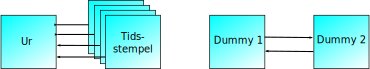
\includegraphics[scale=1]{images/watch-network}
	\caption{Procesnetværk med flere konverteringsprocesser, og analyseprocesser}
	\label{fig:watch_network}
\end{center}
\end{figure}

I \code{greenlets}-versionen skal tidsstempel-processerne vente på at kunne sende sit tidsstempel. Dette gør de ved at oprette en separat tråd  via \code{IO}-dekoratøren. I den separate tråd venter de via funktionen \code{sleep}. Dette er standardmetoden for \emph{greenlets}-versionen når processer ønsker at kunne vente uden at blokere for hele programmet, og er beskrevet på  hjemmesiden for \pycsp. Det medfører dog et overhead at skulle oprette en ny tråd blot for at vente.  Med introduktionen af \code{Wait}, bliver processen lagt på \code{timers}-hoben, og det er derfor ikke længere krævet at oprette en separat tråd til en proces der ønsker at vente. en udvikler der skal planlægge en proces til senere kørsel, slippe derfor i RTP for at skulle introducere \cref{fig:sleep} før en proces kan planlægges.

\begin{lstlisting}[firstnumber=1 ,float=hbtp, label=fig:sleep, caption=Funktion der venter et antal sekunder]
@io
def sleep(n):
    import time
    if n>0: time.sleep(n)
\end{lstlisting}
 
Ved implementeringen af \code{greelets}-versionen, opstår der et problem i opdateringen af uret. begrænsningen om kun at  opdatere uret så længe tidsstemplet er korrekt, har vi implementeret med en \code{alternation}, og en timeout.  Tidsstempel-processen, skal derfor inden et sekund have sendt beskeden til uret, og vil ellers helt droppe forsendelsen. Resultatet af denne implementering kan man se af linje 1 i \cref{tab:watch}. Den gennemsnitlige forsinkelse på 1.529 sekunder burde være umuligt, da opdateringer på over et sekund bør falde bort. Grunden til forsinkelsen ikke falder bort skyldes at tidsstempel-processen korrekt får overført tidsstemplet til urprocessen inden for et sekund. Ur-processen bliver efterfølgende lagt på \code{next} listen da den er klar til at blive kørt. Her skal den så slås med dummy-processerne for at blive udvalgt af \sched en. Når ur-processen bliver udvalgt er tiden forpasset og uret bliver opdateret for sent.
Vi har derfor lavet endnu en version hvor vi også ur-processen efter den har modtaget tidsstemplet kontrollere at tiden ikke er forpasset. Resultatet af denne ændring ses af linje 2 i tabellen, hvor vi kan se at ikke en eneste gang når uret at blive opdateret inden sekundet er forpasset.
\begin{table}[htbp]
	\centering
	\begin{tabular}{l>{\centering\arraybackslash}p{3.1cm}>{\centering\arraybackslash}p{3.1cm}>{\centering\arraybackslash}p{3.1cm}}
       	\toprule
        \mc{Version}     & Rettidige tidsopdateringer&Gennemsnitlig forsinkelse&Standard Afvigelse (SA)\\
        \midrule
        Greenlets ver. 1 & 0  & 1.529 & 0.276 \\
        Greenlets ver. 2 & 0  & NaN   & 0\\
        RTP              & 80 & 0.539 & 0.411 \\
        RTP (50 opdateringer) &100 & 0.077& 0.023\\
        \bottomrule
    \end{tabular}
	\caption[]{Proces-netværk betstående af et ur, 100 opdateringer, og baggrundsprocesser }\\
	\label{tab:watch}
\end{table}

De to forskellige implementeringer af \code{Greenlets}-versionen viser godt hvorfor den ikke er egnet til planlægge processer der er skal aktiveres inden for en tidsperiode. Problemet er at selvom tidsstempel-processerne sender sit data til ur-processen inden for tidsgrænsen. Skal denne stadig kæmpe om at blive aktiveret mod alle dummy-processerne. \Sched en aktiverer processerne ud fra en FIFO strategi, og ur-processen vil derfor komme sidst i køen der ønsker at blive aktiveret. 

I modsætning til \code{greenlets}-versionen, og dens FIFO strategi ser vi i tabellen for RTP-versionen at den  når 80\% af tidsstemplerne. I modsætning til Greenlets-versionen indeholder forsinkelsen kun de tidsstempler der ankom rettidigt. Det mest bemærkseslværdige ved RTP-versionen er SA. Den er meget høj og indikere dermed den gennemsnitlige forsinkelse variere meget. Dette passer ikke sammen med vores forventning om at watch-processen kommer til som den første proces. 


Ved at undersøge de forsinkelsen for de enkelte opdateringen, kunne vi se at de første opdateringerne ankom med en forventet forsinkelse, men igennem  kørte, steg forsinkelsen. Som alternativ til 100 opdatering prøvede vi derfor med 50 opdateringer, og fik et resultat som vi havde forventet. Forsinkelsen de ankommer med er svare til en kørslen af en dummyproces, hvilket er forventet da vi ikke har preemptiv kontekstskift, og derfor nødvendigvis må afslutte en dummyproces før tidsstempel-processen bliver aktiveret. Yderligere undersøgelse sted bestemmer vores problem til prioritetsnedarvning, nærmere bestemt at vi ikke korrekt får nedgraderet ur-processen igen. I dette tilfælde medvirker det til at de efterfølgende tidsstempel-processer fejlagtig modtager en prioritetsnedarvning. Det medfører at antallet af nedarvede prioriteter  hver tidsstempel proces modtager konstant øges.


\section{Konklusion}
